% Тут используется класс, установленный на сервере Papeeria. На случай, если
% текст понадобится редактировать где-то в другом месте, рядом лежит файл matmex-diploma-custom.cls
% который в момент своего создания был идентичен классу, установленному на сервере.
% Для того, чтобы им воспользоваться, замените matmex-diploma на matmex-diploma-custom
% Если вы работаете исключительно в Papeeria то мы настоятельно рекомендуем пользоваться
% классом matmex-diploma, поскольку он будет автоматически обновляться по мере внесения корректив
%

% По умолчанию используется шрифт 14 размера. Если нужен 12-й шрифт, уберите опцию [14pt]
\documentclass[14pt]{matmex-diploma-custom.cls}
\usepackage{enumitem}

%\documentclass[14pt]{matmex-diploma-custom}

\begin{document}
% Год, город, название университета и факультета предопределены,
% но можно и поменять.
% Если англоязычная титульная страница не нужна, то ее можно просто удалить.
\filltitle{ru}{
    chair              = {Кафедра Системного программирования},
    title              = {Телеметрия роботов на базе контроллера TRIK \\ Серверная часть},
    % Здесь указывается тип работы. Возможные значения:
    %   coursework ~--- Курсовая работа
    %   diploma ~--- Диплом специалиста
    %   master ~--- Диплом магистра
    %   bachelor ~--- Диплом бакалавра
    type               = {coursework},
    position           = {студента},
    group              = 244,
    author             = {Свитков Сергей Андреевич},
    supervisorPosition = {старший преподаватель},
    supervisor         = {Литвинов Ю.\,В.},
%   reviewerPosition   = {ст. преп.},
%   reviewer           = {Привалов А.\,И.},
%   chairHeadPosition  = {д.\,ф.-м.\,н., профессор},
%   chairHead          = {Хунта К.\,Х.},
%   university         = {Санкт-Петербургский Государственный Университет},
%   faculty            = {Математико-механический факультет},
%   city               = {Санкт-Петербург},
%   year               = {2013}
}
%\filltitle{en}{
%    chair              = {The Meaning of Life \\ Uselessness of Everything},
%    title              = {Empty subset as closed set},
%    author             = {Edelweis Mashkin},
%    supervisorPosition = {professor},
%    supervisor         = {Amvrosy Vibegallo},
%    reviewerPosition   = {assistant},
%    reviewer           = {Alexander Privalov},
%    chairHeadPosition  = {professor},
%    chairHead          = {Christobal Junta},
%}
\maketitle
\tableofcontents
% У введения нет номера главы
\section*{Введение}

В последние годы область робототехники развивается очень быстро, появляется множество робототехнических конструкторов.


Одним из них является TRIK \cite{trik} --- кибернетический конструктор с центральным процессором на базе ARM и операционной системой на базе ядра Linux. Модели роботов TRIK применяются как для обучения школьников, так и для серьезных соревнований, например, WRO (World Robot Olympiad), проходившей в Сочи (2014г); Ежегодный фестиваль робототехники Робофинист (2015г). Роботы моделей TRIK имеют ряд датчиков, таких как гироскоп, акселерометр, датчик заряда батареи. Так же робот предоставляет сетевой интерфейс Wi-Fi.

Но сам по себе робот, без программ на нем, представляет малый интерес. Следует сказать, что исполнение программ на роботе происходит в реальном времени, поэтому очень важной является возможность отслеживать показания датчиков робота во время работы приложений.

Кроме того, необходимо учитывать, что соединение Wi-Fi с роботом нестабильно, и его легко перегрузить, поэтому алгоритм обмена сообщениями между роботом и ПК пользователя\footnote{В данном случае речь идет о клиентском приложении, запущенном на персональном компьютере пользователя. В дальнейшем --- клиент} должен обеспечивать минимальную задержку между снятием показаний с датчиков робота и их визуализацией в клиентском приложении, но при этом обеспечивать минимальную потерю данных.

Поэтому задача разработки эффективного алгоритма для телеметрии данных, получаемых с датчиков робота, является актуальной и важной.

\subsection*{Постановка задачи}
Поскольку задача телеметрии роботов модели TRIK была решена ранее Матвеем Брыксиным в рамках его курсовой работы, то целью данной работы является разработка нового алгоритма передачи данных с робота на ПК и последующее сравнение нового алгоритма с существующим, а так же рефакторинг уже написанного кода.

Для достижения данной цели были поставлены следующие задачи:
\begin{enumerate}
\item добавить поддержку передачи данных с использованием протокола UDP

\item провести сравнение эффективности существовашего ранее решения и решения, полученного в ходе данной работы

\item провести рефакторинг кода
\end{enumerate}

\section{Обзор}

\subsection{Обзор существующих решений}
Был проведен обзор существующих решений задачи телеметрии роботов в различных условиях.

\subsubsection*{A Comparison of Lightweight Communication Protocols in Robotic Applications \cite{comp}}
В данной работе рассказывается о сравнении двух легковесных протоколов передачи данных с робота : CoAP \cite{coap} и MQTT-SN \cite{mqtt}.

Статья, написанная по данной работе, была полезна тем, что в ней описан подход к сравнению двух протоколов.

\subsubsection*{A Data-Rate Aware Telemetry Scheduler \cite{datarate}}
В данной статье описан подход к реализации телеметрии в условиях очень плохого соединения с роботом.

Для решения задачи телеметрии в таких условиях автор статьи предлагает использовать алгоритм приоретизации сообщений в зависимости от их важности.

Но данный подход не может быть использован, поскольку это не соответствует требованиям системы реального времени.

\subsubsection*{Телеметрия моделей ТРИК \cite{m}}
Данная работа рассказывает о реализации телеметрии моделей TRIK. Передача данных с робота осуществляется по протоколу TCP с заранее объявленным интервалом.

Решение автора было взято в качестве основы с целью улучшить его. 

\subsection{Итог}
Сформулирована гипотеза о том, что передача части данных по UDP уменьшит задержку при визуализации данных и при этом практически не повлияет на качество визуализации.

В связи с этим было принято решение переиспользовать существующий код, внеся в него следующие изменения:
\begin{enumerate}  
\item добавить возможность передачи данных с датчиков робота с использованием протокола UDP 
\item разработать алгоритм передачи данных с использованием комбинации протоколов TCP и UDP
\item провести рефакторинг
\end{enumerate}

\section{Реализация} 
Основным моментом в реализации решения задачи являются использование UDP в комбинации с TCP.
\subsection{UDP + TCP}
UDP, в отличие от TCP, не гарантирует доставку всех пакетов, передаваемых по сети с одного устройства на другое. В связи с этим фактом UDP не может быть использован для передачи важных сообщений --- в данном случае такими сообщениями будем считать сигналы о старте телеметрии и о ее завершении. Однако такие сообщения передаются редко в сравнении с частотой отправки основного типа сообщений, отправляемых с робота на клиент --- сообщений, содержащих в себе показания датчиков робота. 

Так как сообщение с показаниями датчиков отправляется каждые 10 мс, тот факт, что при передаче может быть утеряно некоторое количество пакетов, не является критичным. Следует отметитить, что потеря пакетов, как показали исследования, случается довольно редко и в небольших количествах.

Поэтому UDP можно считать оптимальным для оптимизации протокола передачи данных, но, как было отмечено выше, использование только UDP может привести к потере важного сигнала, что может плохо отразиться на работе системы.

\subsection{Программное решение}
Был написан класс для реализации обмена сообщениями между сервером и клиентом по протоколу UDP. Кроме того, был добавлен интерфейс, в который вынесены общие методы для классов, реализующих UDP и TCP.

Итоговый вариант архитектуры \cite{gof}: \ref{overflow1}
\begin{figure*}
\centering
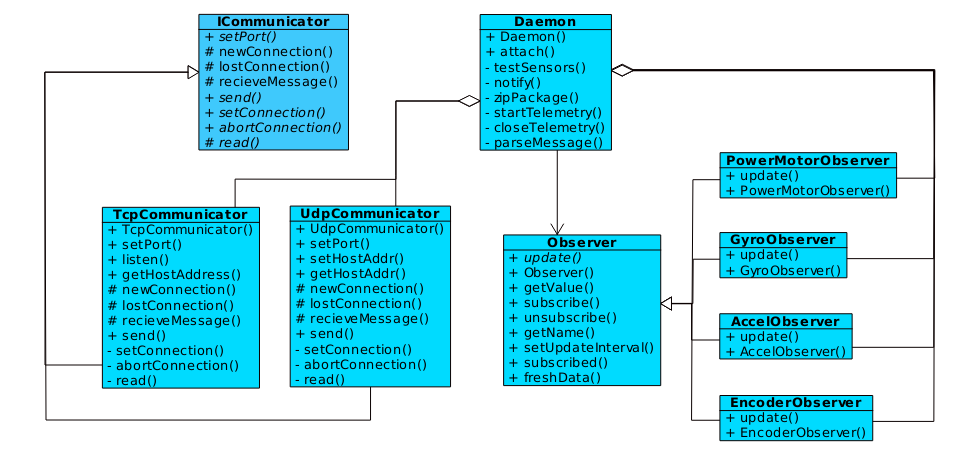
\includegraphics[width=\textwidth]{serv.png}
\caption{Архитектура \label{overflow1}}
\end{figure*}

\section{Исследования}
С целью проверки гипотезы, выдвинутой в начале данной работы, был проведен ряд исследований с целью сравнить исходный вариант протокола с разработанным в рамках данной работы.

Следует отметить, что радиус покрытия Wi-Fi сети робота --- около 20 метров\footnote{Выявлено опытным путем}, поэтому было принято решение проводить исследования в условиях удаленности ПК с запущенным клиентом от робота на расстояние около 10 метров.

Критерии, по которым проводилось сравнение протоколов:
\begin{enumerate}  
\item величина задержки между моментом снятия показаний датчиков робота и моментом их визуализации на клиенте
\item количество теряемых пакетов
\item то, насколько негативно использование протокола влияет на визуализацию
\end{enumerate}

\subsection{Сравнение времени задержки}
Было решено сравнить количество времени\footnote{В таблице --- среднее время}, за которое происходит считывание, отправка, парсинг и визуализация 1000 пакетов для протоколов TCP и комбинации TCP + UDP. Результаты представлены в таблице \ref{tab:table1}
\begin{table}
\centering
  \caption{Результаты замеров}
  \label{tab:table1}
  \begin{tabular}{|p{3 cm}|p{3 cm}|p{3 cm}|p{3 cm}|}
    \hline
    Используемый протокол & Среднее время, мс & Среднее количество потерянных пакетов, \% & расстояние до робота\\
    \hline
    TCP & 51100 & 0 & 10\\
    \hline
    TCP + UDP & 44600 & 0 & 10\\
    \hline
    TCP & 59200 & 0 & 15 \\
    \hline
    TCP + UDP & 43500 & 7 & 15\\
    \hline
  \end{tabular}
\end{table}

Как можно заметить из результатов таблицы, средняя задержка для одного пакета на нормальном расстоянии (10 м) при использовании TCP составляет около 51 мс, а средняя задержка для одного пакета при использовании предложенного в статье алгоритма, соответственно, около 44 мс. Из данных результатов можно сделать вывод о том, что задержка при использовании TCP + UDP в среднем уменьшается на 14\%. 

Задержка же при расстоянии 15 м для протокола TCP становится больше, поскольку сигнал становится более слабым и TCP приходится досылать те пакеты, которые не были досланы до пользователя.
\subsection{Сравнение визуализации}
Поскольку потеря пакетов в нормальных условиях соединения практически не происходит, использование UDP в качестве протокола для передачи данных датчиков практически не окажет влияния на визуализацию.

Для доказательства этого приводятся графики показаний акселерометра \ref{overflow4} \ref{overflow5}

\begin{figure*}
\centering
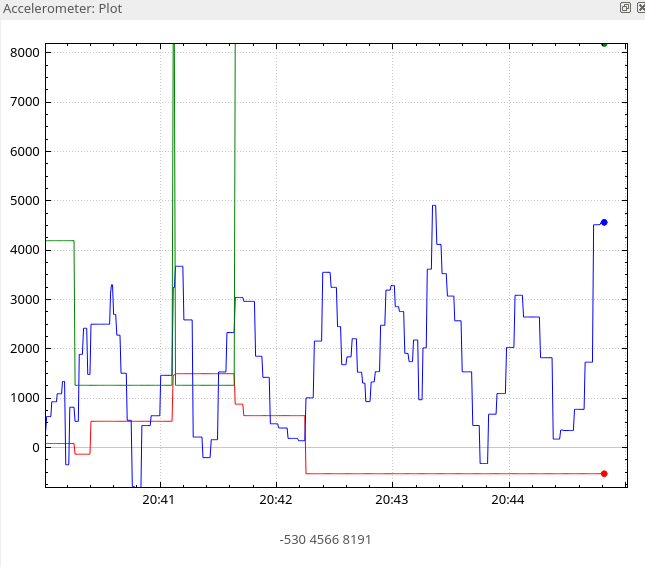
\includegraphics[width=\textwidth]{tcp.png}
\caption{Фрагмент графиков, TCP \label{overflow4}}
\end{figure*}

\begin{figure*}
\centering
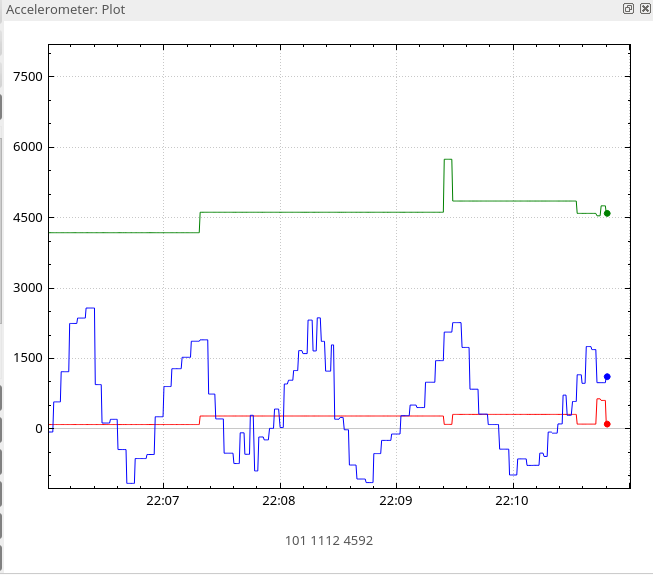
\includegraphics[width=\textwidth]{tcpudp.png}
\caption{Фрагмент графиков, TCP + UDP \label{overflow5}}
\end{figure*}

\subsection{Другие возможные исследования}
Следует отметить, что были предложены и другие варианты протоколов для сравнения с TCP + UDP, например:
\begin{enumerate}
\item протокол, использующий TCP, но при этом не посылающий каждый пятый пакет с данными
\item протокол, использующий TCP, но посылающий пакеты с данными в два раза реже
\end{enumerate}

Данные варианты не были рассмотрены, поскольку никак не могут повлиять на задержку и лишь негативно сказываются на визуализации данных.

\subsection{Итог}
По результатам сравнения можно утверждать, что разработанное в рамках данной курсовой работы решение является более эффективным чем то, что было предложено ранее.

\section{Рефакторинг}
Код, на основе которого проводилась данная работа, обладал рядом недостатков, которые были исправлены.
Исправленные недостатки:
\begin{enumerate}
\item объявление нескольких классов в одном файле
\item cyclic dependency
\item неуместное совместное использование forward declaration и include в .h файлах 
\item использование using namespace в .h файлах
\end{enumerate}


\section*{Заключение}
В ходе исследований, проведенных в рамках данной работы было выявлено,что предложенный протокол передачи данных, использующий TCP + UDP, является более эффективным в рамках конкретной задачи, поэтому результатом данной работы можно считать улучшение алгоритма обмена сообщениями между роботом и клиентом, выражающееся в виде уменьшения задержки между отправкой пакета с данными и визуализацией данных на 14\% и рефакторинг кода.

По результатам работы был сделан доклад на конференции SEIM-2016.

\subsection*{Дальнейшие перспективы}
В дальнейшем планируется закончить оформление кода, полученного в ходе данной работы, в соответствии со стайлгайдом \cite{guide} TRIK.

\setmonofont[Mapping=tex-text]{CMU Typewriter Text}
\bibliographystyle{ugost2008ls}
\bibliography{coursework.bib}
\end{document}
